\documentclass[a4paper, 10pt,twoside]{article}
\usepackage[utf8x]{inputenc}

% english language
\usepackage[UKenglish]{babel}

% ps tricks
\usepackage[usenames,dvipsnames]{pstricks}

% about title
\usepackage{titlesec}
\usepackage{hyperref}
\usepackage{url}

% margins
\topmargin 0cm
\headsep 1cm
\headheight 0.6cm
\textwidth 16.6cm
\textheight 21.8cm
\evensidemargin -0.5cm
\oddsidemargin -0.5cm

% mathematics
\usepackage{amsmath}
\usepackage{amsfonts}


% definition
\usepackage{amsthm}
\theoremstyle{plain}
\newtheorem{thm}{Theorem}[section]
\newtheorem{cor}[thm]{Proof.}

\theoremstyle{definition}
\newtheorem{defn}{Definition}[section]

\theoremstyle{remark}
\newtheorem{rmk}{Remark}

% test format
\usepackage{verbatim}
\usepackage{color}
\usepackage{eurosym}

% symbols
\usepackage{textcomp, latexsym, amssymb, gensymb, placeins}
\usepackage[mathscr]{euscript}
\usepackage{amsmath}

% figures
\usepackage{epsfig}
\usepackage{graphics, epsfig, color, colortbl, supertabular}
\usepackage{subfigure}
\usepackage{epstopdf}

% tables
\usepackage{multirow, ctable, rotating, lscape}
\usepackage{array}
\usepackage{booktabs}
\usepackage{supertabular}
\usepackage{tabularx}
\usepackage{graphicx}
\usepackage{IEEEtrantools}
% other packages
\usepackage{hyperref}
\def\thesection{\arabic{section}}
\def\theequation{\arabic{equation}}

\addtocounter{section}{1}
\setcounter{secnumdepth}{3}
\setcounter{tocdepth}{3}
\setcounter{section}{0}

\usepackage{float}
\usepackage{stmaryrd}


% tikz
\usepackage{tikz}
\usetikzlibrary{mindmap,trees}
\usetikzlibrary{arrows,decorations.pathmorphing,backgrounds,fit,positioning,%
  shapes.symbols,chains}
\usetikzlibrary{calc,trees,positioning,arrows,chains,shapes.geometric,%
  decorations.pathreplacing,decorations.pathmorphing,shapes,%
  matrix,shapes.symbols}


% acronyms
\usepackage{acronym}


% URL
\usepackage{url}

\usepackage{fancyhdr}
\usepackage{etex}
\usepackage{epstopdf}

% X Quartapelle
% \renewcommand{\theequation}{\thechapter.\arabic{equation}}
% \newcommand{\clearemptydoublepage}{\newpage{\pagestyle{empty}
% \cleardoublepage}}
\renewcommand{\headrulewidth}{0.3pt}
\renewcommand{\footrulewidth}{0.3pt}
\newcommand{\virgolette}[1]{``#1''}

% Mathematical Operator
\newcommand{\WeNT}{\widehat{\mathcal{W}}}
\newcommand{\W}{$\mathcal{W}$}
\newcommand{\LE}{\mathcal{L}}
\newcommand{\Lne}{$\mathcal{L}$}
\newcommand{\delOp}{\widehat{\boldsymbol{\nabla}}}
\newcommand{\diver}[1]{\text{Div}\big(#1\big)}
\newcommand{\invariants}{$\big(I_{\C},II_{\C},III_{\C}\big)$}

% Eucledian spaces
\newcommand{\Real}{$\mathbb{R}^3$}
\newcommand{\RN}{\mathbb{R}^{N_h}}

% Lagrangian and Eulerian displacements
\newcommand{\displL}{\widehat{\underline{\eta}}}
\newcommand{\displE}{\underline{\eta}}

% Discrete displacement, velocity and acceleration
% The fist command is to reuse the same already existing formula
\newcommand{\Spost}{\widehat{\underline{\Lambda}}}
\newcommand{\GradSpost}{\delOp\delta\Spost}
\newcommand{\vectL}{\widehat{\underline{\Lambda}}}
\newcommand{\velVect}{\widehat{\underline{W}}}
\newcommand{\acc}{\widehat{\underline{A}}}

% Stiffness Vectors, discretized system
\newcommand{\StiffVect}{\underline{K}(\vectL)}
\newcommand{\StiffDiscr}[1]{\underline{K}(\vectL^{#1})}

% Lagrangian velocity
\newcommand{\velL}{\widehat{\underline{v}}}
\newcommand{\velE}{\underline{v}} %Test function (velocity)
\newcommand{\velwE}{\widehat{\underline{w}}}

% Programming names
\newcommand{\SSol}{\textit{Structural Solver}}
\newcommand{\SSolNC}{Structural Solver}
\newcommand{\lv}{\texttt{LifeV}\space}
\newcommand{\tPC}[1]{\texttt{#1}}
\newcommand{\AES}{AssemblyElementalStructure}
\newcommand{\tSS}{\textit{test\_structuralsolver}}

% Reference and Current Configuration
\newcommand{\RefCon}{$\mathcal{B}_0$}
\newcommand{\CurCon}{$\mathcal{B}(t)$}
\newcommand{\RefConE}{\mathcal{B}_0}
\newcommand{\CurConE}{\mathcal{B}(t)}

% Position in the reference and current configuration
\newcommand{\posE}{\underline{X}}
\newcommand{\nposE}{\underline{x}}
\newcommand{\pos}{$\underline{X}$}
\newcommand{\npos}{$\underline{x}$}

% Tensors and matrices
\newcommand{\F}{\textbf{F}}
\newcommand{\cofF}{\text{Cof}\textbf{F}}
\newcommand{\T}{\textbf{T}}
\newcommand{\D}{\textbf{D}}
\newcommand{\C}{\textbf{C}}
\newcommand{\Cbar}{\bar{\textbf{C}}}
\newcommand{\I}{\textbf{I}}
\newcommand{\mass}{\textbf{M}}
\newcommand{\Piola}{\textbf{P}}
\newcommand{\Et}{\textbf{E}}

\newcommand{\Eqref}[1]{Eq.~\eqref{#1}}
\newcommand{\secref}[1]{Sec.~\ref{#1}}
\newcommand{\chref}[1]{Ch.~\ref{#1}}
\newcommand{\appref}[1]{Appendix~\ref{#1}}
\newcommand{\sectionref}[1]{Section~\ref{#1}}
\newcommand{\tworef}[2]{Secs.~\ref{#1}~and~\ref{#2}}
\newcommand{\tabref}[1]{Tab.~\ref{#1}}
\newcommand{\figRef}[1]{Fig.~\ref{#1}}
\newcommand{\figsRef}[2]{Figs.~\ref{#1}~and~\ref{#2}}

\newcommand{\nor}{\boldsymbol{n}}
\newcommand{\disM}{\widehat{\boldsymbol{d}}}
\newcommand{\disF}{\widehat{\boldsymbol{d}}_{\mathcal{F}}}
\newcommand{\flDomain}{\mathcal{F}}
\newcommand{\disS}{\boldsymbol{D}}
\newcommand{\velocityM}{\widehat{\boldsymbol{v}}}
\newcommand{\velFl}{\boldsymbol{u}}
\newcommand{\velFlv}{\boldsymbol{v}}
\newcommand{\ALEvel}{\boldsymbol{w}_{\mathcal{F}}}
\newcommand{\velocityS}{\boldsymbol{v}}
\newcommand{\accelM}{\widehat{\boldsymbol{a}}}
\newcommand{\accelS}{\boldsymbol{a}}
\newcommand{\test}{\boldsymbol{\phi}}
\newcommand{\testE}{\boldsymbol{\phi}}
\newcommand{\testVE}{\widehat{\boldsymbol{\psi}}}
\newcommand{\zero}{\boldsymbol{0}}
\newcommand{\tri}{\mathcal{T}_h}

\newcommand{\iso}{\texttt{isotropic}}
\newcommand{\aniso}{\texttt{anisotropic}}
\newcommand{\isoWe}{\overline{\mathcal{W}}}
% Expression for the Exponential-Material
\newcommand{\term}{e^{\gamma\left(I_{\C}-3\right)}}
\newcommand{\Ue}{\mathcal{U}}

% Title Page
\title{Structure module in \textit{LifeV}: Organization, Constitutive models, and Examples}
\author{Paolo Tricerri}

\begin{document}
\bibliographystyle{IEEEtran}
\bstctlcite{myctlfullname}

\maketitle

\section*{Summary}
This document describes the organization of the Structure module of LifeV 3.8.5 (released in May 2014). In particular, it provides the list of the different constitutive models currently available, it presents the classes implemented in the module, their hierarchy, and  interactions. In addition, the list of the different example folders is provided together with a small description for each of them. This document does not deal with the continuum mechanics theory needed to define all the scalar, vectorial, and tensorial quantities that appear in the constitutive models; the interested reader may refer to \cite{book::Holzapfel2000}.

\section{Constitutive models}
The constitutive models in LifeV are grouped in two sub-folders, called \texttt{isotropic} and \texttt{anisotropic}, of the folder \texttt{lifev/structure/solver}. The folder named \iso\space contains the isotropic strain energy functions, while the one called \texttt{anisotropic}\space contains the strain energy functions for the single family of fibers that can be used in transversely isotropic and anisotropic constitutive models such as the ones discussed in \cite{thesis::Tricerri}. For the mathematical definition of a transversely isotropic material as well as for the one of an anisotropic material, the interested reader my refer to \cite{book::Holzapfel2000}. For most of the constitutive models available in \lv, the strain energy function is formulated according to the additive volumetric-isochoric split as consequence of the volumetric-isochoric multiplicative decomposition of the deformation gradient tensor as proposed in \cite{paper::Flory1956} and done in \cite{thesis::Tricerri}. Therefore,most the constitutive laws are formulated in order to simulate the nearly incompressible behavior of arteries; however, two isotropic laws are formulated in the compressible form \cite{book::Holzapfel2000,thesis::Tricerri}. Hereafter, we firstly present the isotropic laws in the compressible form, secondly the isotropic laws for the simulation of the quasi-incompressible behavior of arteries, and finally the strain energy functions for the single family of fibers. In the following, the strain energy function is indicated as $\WeNT$ and the invariants of the right Cauchy-Green tensor \C\space are indicated as $I_{1}$,$I_{2}$,$I_{3}$ \cite{book::Holzapfel2000}.

\paragraph{Isotropic models in the compressible form}
\begin{itemize}
\item St.Venant Kirchhoff model for small deformations (i.e. linear elastic model) (see \cite{thesis::Crosetto}) for the definition of the first Piola-Kirchhoff tensor.
\item St.Venant Kirchhoff model for finite deformations
  \begin{equation}
    \displaystyle \WeNT \left(I_1,I_2\right) = \left( \frac{\lambda}{8} + \frac{\mu}{4} \right)I_1^2 - \left( \frac{3}{4}\lambda + \frac{\mu}{2} \right)I_1 - \frac{\mu}{2}I_2 + \frac{9}{8}\lambda + \frac{3}{4}\mu
    \label{SVKcompr}
  \end{equation}
\end{itemize}
\paragraph{Isotropic models in the nearly-incompressible form}
\begin{itemize}
\item First order exponential
  \begin{equation}
    \displaystyle \isoWe\left( \overline{I}_1, \overline{I}_2\right) = \displaystyle \frac{\alpha_1}{2\gamma_1}\bigg( \text{e}^{\gamma_1( \overline{I}_1-3)} - 1\bigg)
        \end{equation}
\item Second order exponential
  \begin{equation}
    \displaystyle \isoWe\left( \overline{I}_1, \overline{I}_2\right) = \displaystyle  \frac{\alpha_2}{2\gamma_2}\bigg( \text{e}^{\gamma_2( \overline{I}_1-3)^2} - 1\bigg)
  \end{equation}
\item Neohookean
  \begin{equation}
    \displaystyle \isoWe\left( \overline{I}_1, \overline{I}_2\right) = \displaystyle \frac{\mu}{2}\left( \overline{I}_1 - 3 \right)
  \end{equation}
\item St. Venant-Kirchhoff (isochoric formulation)
  \begin{equation}
    \displaystyle \isoWe\left( \overline{I}_1, \overline{I}_2\right) = \displaystyle \left( \frac{\lambda}{8} + \frac{\mu}{4} \right)\overline{I}_1^2 - \left( \frac{3}{4}\lambda + \frac{\mu}{2} \right)\overline{I}_1 - \frac{\mu}{2}\overline{I}_2 + \frac{9}{8}\lambda + \frac{3}{4}\mu
    \label{SVKni}
  \end{equation}
\end{itemize}
For a discussion about the physical meaning of the different material parameters $\lambda,\mu,\alpha_1,\gamma_1,\alpha_2,\gamma_2$ in Eqs.~\eqref{SVKcompr}-\eqref{SVKni}, the interested reader may refer to \cite{book::Holzapfel2000}.
\paragraph{Strain energy function for the single family of fibers}: in the following, we assume that the local alignment of the fibers belonging to the $i$-th family (for $i=1\ldots N$ being $N$ the number of families of fibers considered in the material \cite{book::Holzapfel2000}) can be described by a vectorial field (either defined analytically on the computational domain or read from file) for which the structural tensor associated to the single family of fibers \cite{book::Holzapfel2000} can be defined. Consequently, here we assume that all the invariants needed to define the strain energy functions are well defined in the computational domain. The strain energy functions are:
\begin{itemize}
\item Second order exponential along the fiber direction with activation at zero strain (with reference stretch for the fibers equal to one)
  \begin{equation}
    \displaystyle \isoWe^{(i)}\left( \overline{I}_4 \right) = \displaystyle  \frac{\alpha^{(i)}}{2\gamma^{(i)}}\bigg( \text{e}^{\gamma^{(i)}( \overline{I}_4^{(i)}-1)^2} - 1\bigg)
    \label{singleFour}
  \end{equation}
\item Second order exponential along the fiber direction with activation at finite stretch $I_4^{A}$
  \begin{equation}
    \displaystyle \isoWe^{(i)}\left( \overline{I}_4;I_4^{A} \right) = \displaystyle  \frac{\alpha^{(i)}}{2\gamma^{(i)}}\bigg( \text{e}^{\gamma^{(i)}( \overline{I}_4^{(i)}-I_4^{A})^2} - 1\bigg)
  \end{equation}
\item Second order exponential with distributed collagen fibers with activation at zero strain (with reference stretch for the fibers equal to one)
  \begin{equation}
    \displaystyle \isoWe^{(i)}\left( \overline{I}_1,\overline{I}_4 \right) = \displaystyle  \frac{\alpha^{(i)}}{2\gamma^{(i)}}\bigg( \text{e}^{\gamma^{(i)}( \kappa \overline{I}_1 + (1-3\kappa)\overline{I}_4^{(i)}-1)^2} - 1\bigg)
  \end{equation}
\item Second order exponential along the fiber direction with activation at finite stretch to use in the multi-mechanism model proposed in \cite{thesis::DalongLi}
  \begin{equation}
    \displaystyle \isoWe^{(i)}\left( \overline{I}_4^{t_A,(i)} \right) = \displaystyle  \frac{\alpha^{(i)}}{2\gamma^{(i)}}\bigg( \text{e}^{\gamma^{(i)}( \overline{I}_4^{t_A,(i)}-1)^2} - 1\bigg),
    \label{multimechSingle}
  \end{equation}
  where $\overline{I}_4^{t_A,(i)}$ indicates that the fourth invariant associated to the right Cauchy-Green and the $i$-th structural tensor \cite{book::Holzapfel2000} must be referred to the activation configuration (reached at a certain time $t_A$) of the $i$-th family of fibers. It is worth pointing out that, although the multi-mechanism model proposed in \cite{thesis::DalongLi} has been implemented in \lv and successfully used in the case of homogeneous deformations (e.g. traction of a cube) numerical issues such as stagnation of the Newton method must be reported for more general, i.e. in-homogeneous, deformations; see the discussion in \cite{thesis::Tricerri}.
\end{itemize}

\paragraph{Volumetric strain energy function}: this strain energy function is employed to penalize the deformations that would lead to changes in the volume of the continuous body under consideration \cite{book::Holzapfel2000,thesis::Tricerri}. The strain energy function implemented in \lv is:
\begin{equation}
  \displaystyle \Ue(J) = \frac{K}{4}\left( (J-1)^2 +\text{ln}^2(J)\right)
  \label{volumStrain}
\end{equation}
where $J$ is the volume ratio, i.e. the determinant of the deformation gradient tensor \cite{book::Holzapfel2000}, and $K$ is the penalization parameter that has to be set ``high enough'' to ensure the nearly-incompressible behavior of the material.

\section{Organization}
\texttt{LifeV} \cite{LifeV} is a parallel finite element \texttt{C++} library that implements state of the art of mathematical models and numerical methods for the solution of three-dimensional partial differential equations. \texttt{LifeV} targets a broad audience of researchers; for this reason, the organization and implementation of the different constitutive models have been driven by necessity of having  a ``user-oriented'' library. It includes numerical methods and algorithms for the numerical simulation of complex engineering problems; indeed it has been extensively used for the numerical simulation of the human cardiovascular system, see e.g. \cite{thesis::Crosetto,thesis::Malossi}, porous media, cardiac tissue, and other physical systems such as, for instance, free surface flows in orbitally shaken reactors \cite{thesis::Quinodoz}. The main features of the structure module are flexibility and computational efficiency.

Flexibility has been achieved thanks to the implementation of a unified framework for the numerical simulations of structural mechanics problems. The organization of the structure module is depicted in \figRef{organization}. The numerical solution of the arterial wall mechanics is managed by the \textit{Solver Class} which, for instance, executes the Newton-Raphson method. As represented in \figRef{organization}, dynamic structural mechanics problems can be simulated thanks to the integration of the tools implementing time advancing schemes such as Backward Difference Formula (BDF) methods \cite{book::QSS00}, provided by the core module of the library, inside the structure module.  The different constitutive models have been implemented according to the so-called \textit{Factory pattern} design described in \cite{book::DesignPattern} which provides a way to encapsulate a group of individual classes (see \cite{book::Cplus}), each of them representing a single constitutive model, that have a common theme through a common abstract interface, implemented in an abstract class, the \textit{Constitutive Model Class} in \figRef{organization}. Such abstract class can be used by external classes, such as the \textit{Solver Class}, to solve the structural mechanics problem. The \textit{Solver Class} creates an instance of the \textit{Constitutive Model Class} \cite{book::Cplus} and then uses the generic interface of the \textit{Constitutive Model Class} to create the instance of the chosen constitutive model among the ones that are available. This pattern separates the details of implementation of a set of objects, i.e. constitutive models, from their general usage and relies on object composition \cite{book::DesignPattern}. Such organization of the structure module has led to a unified and flexible environment where each term of the strain energy function, i.e. the volumetric, the isochoric isotropic and, possibly, the isochoric model for the single family of fibers, can be freely chosen by choosing a set of parameters when the simulation is started. The hierarchical relation between the different implementations of the constitutive models and the \textit{Solver Class} is represented in \figRef{organization}. As a final remark, as represented in \figRef{organization}, the material parameters for the selected constitutive laws modeling the tissue are handled by the \textit{Material Parameter Class} which is contained in the abstract interface \textit{Constitutive Model Class}.
\begin{figure}[t!]
  \centering
  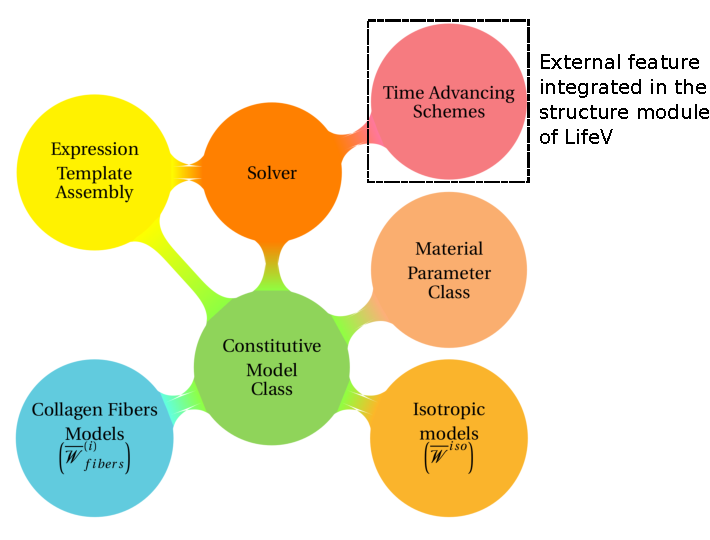
\includegraphics[height=8cm]{schemePdf.pdf}
  \caption{Organization of the structure module of the finite element library \texttt{LifeV}}
  \label{organization}
\end{figure}
When considering nonlinear constitutive models for the arterial tissue, the numerical simulation of the arterial wall deformations under the action of external forces requires the numerical solution of a highly nonlinear systems of equation. The nonlinear systems are solved by means of the Newton-Raphson method which requires the repeated evaluation of the tangent matrix of the stiffness matrix and variational residual of the Newton-Raphson method \cite{thesis::Tricerri}. From the computational point of view, these two operations are among the most expensive ones together with the solution of the linearized problem by means of iterative methods (e.g. GMRES \cite{paper::Saad}); for this reason, as discussed in \cite{thesis::Quinodoz,thesis::Andreas}, the implementation of efficient routines to assemble either the tangent stiffness matrix, i.e. $\mathcal{\boldsymbol{J}}_{\Piola}\left( \disM_h^k \right)\left(\testVE_B,\testVE_A\right)$, and the residual vector $\mathcal{R}\left( \disM_h^k \right)\left( \testVE_{h,A}\right)$ is extremely important. The computational efficiency of the structure module has been achieved by means of the implementation of the finite element assembly routines for $\mathcal{\boldsymbol{J}}_{\Piola}\left( \disM_h^k \right)\left(\testVE_B,\testVE_A\right)$ and $\mathcal{R}\left( \disM_h^k \right)\left( \testVE_{h,A}\right)$ in the framework for finite element assembly, based on template meta-programming \cite{paper::Veneziani}, described in \cite{thesis::Quinodoz}. Such framework is not detailed here; however, it is worth pointing out that, the work of \cite{thesis::Quinodoz}, initially developed for fluid dynamics applications, has been deeply extended in order to include the possibility of finite element assembly routines for structural mechanics problems. From the implementation point of view, the routines for the finite element assembly of the matrices and vectors have been implemented in the \textit{Expression Template Assembly} framework indicated in \figRef{organization}; the correct execution of the assembly routines is controlled by the \textit{Solver Class} and the \textit{Constitutive Model Class}, as represented in \figRef{organization}. % Although the current efficient implementation of the finite element assembly, other types of assembly routines can be found in literature \cite{book::Hughes}. In order to highlight the relevance of the implementation efforts carried out in this work, in \secref{validazio}, a comparison of the computational times needed to assemble the linearized operator of \Eqref{matrixOperator} when employing two different methodologies for the finite element assembly is presented.

\section{Example folders}
\begin{enumerate}
\item \texttt{example\_creatingDamagedZone}. It changes the volume flag of the tetrahedra (or, possibly hexahedra depending on RegionMesh capabilities) contained in the intersection between the computational domain under consideration and the sphere of center and radius defined in the main.cpp of the test.
\item \texttt{example\_anisotropicTraction}. It implements a dynamic structural mechanics problem in which isotropic and anisotropic laws can be employed. Three sets of boundary conditions for traction, inflation, and shear tests are already defined.
\item \texttt{example\_partitionMesh}. It uses the Offline Partitioning Tool to partition a mesh offline. This example has been created from the partition\_io test adding variables to easily import and export the meshes under consideration.
\item \texttt{example\_computationNorm}. It shows how to compute the $\text{L}^2$ or $\text{H}^1$ error of a numerical solution with respect to an analytic solution.
\item \texttt{example\_evaluatingScalarVectorialTensorialQuantitiesUsingETA}. In this example, a numerical solution is read from an hdf5 file and scalar, vectorial, and tensorial quantities (such as the volume ratio $J$, the deformed vectors of the collagen fibers, or the components of the deformation gradient tensor) are computed using the evaluation tree based on the expression template framework \cite{thesis::Quinodoz}.
\item \texttt{example\_computePrincipalTensions}. In this example, the components of the Cauchy stress tensor is computed from a numerical solution contained in a hdf5 file.
\item \texttt{example\_checkingFibersDirection}. This example has been created in order to check the definition of the local alignment collagen fibers on different types of domains.
\item \texttt{example\_bodyForces}. This example solves a structural mechanics problem with a body force term at the right hand side of the conservation equation of linear momentum.
\end{enumerate}
\bibliography{references}

\end{document}
